\chapter{Técnicas de detección}\label{TECNICAS_DE_DETECCION}
El hombre ha realizado diversos experimentos científicos de aceleradores de partículas, como el Gran Colisionador de Hadrones o LHC (Large Hadron Collider) ésto con la finalidad de acelarar las partículas para que colisionen entre sí y generar subproductos que, al estudiarlos, nos dan un idea más clara del mundo subatómico, sin embargo, sólo puede llegar a energías limitadas, alrededor de los TeV. Es por ello que radica la importancia del estudio de astropartículas, su origen galáctico y como estos se relacionan a eventos de gran magnitud, como remanentes de supernovas, núcleos activos de galaxias, agujeros negros entre otros. Estos eventos son considerados fuentes naturales de aceleadores de partículas y llegan a energías desde los TeV hasta los EeV \cite{Gonzales}. En contra parte, los rayos cósmicos y los rayos gamma son muy difíciles de detectar debido a sus interacción con moléculas de la atmósfera, debido a ésto se utilizan diversas técnicas para su detección que las clasificaremos en directas e indirectas:
\section{Directas}
	Con el objetivo de mejorar la forma de detección de estas partículas se consideró un opción de utilizar telescopios espaciales para que éstos logren detectarlos sin que hayan interaccionado con la atmósfera, sin embargo ésto conlleva a una desventaja, y es que su área de detección es pequeña ya que debe ser llevada al espacio. Uno de los más famosos, es el Telescopio de Área Grande Fermi o Fermi-LAT que posee un área efectiva de detección $80 m^2$ y trabaja en un rango de energía de 20 MeV hasta arriba de los 1TeV, obteniendo su dirección, tiempo de llegada y su energía \cite{Abdollahi_2020}.
\section{Indirectas}
	Otro técnica de detección es utilizando justamente la interacción de los rayos cósmicos y gamma con la atmósfera, que por medio de la radiación producido por partículas que viajan a velocidades más altas que la luz en un medio dejan un rastro azulado conocida como Efecto Cherenkov (ver sec \ref{EFECTO_CHERENKOV}), ésta luz es la detectada por los observatorios que se han construido en la superficie terrestre. Uno de ellos son los telescopios que captan ésta señal dejada, llamados Telescopios de imágenes de aire Cherenkov: IACT's \cite{Wild}; uno de los más reconocidos actualmente debido a su tecnología y área detección es el CTA (Cherenkov Telescope Array) que está conformado por 100 telescopios repartidos en el hemisferio norte y sur (España y Chile respectivamente) que trajará en un rango energértico de entre los 20 GeV a 300 TeV.
	
	De igual forma se han construido observatorios conformados por arreglos de tanques que contienen en su interior agua ultra pura donde se produce el efecto Cherenkov, siendo uno de los más importantes HAWC (High Altitude Water Cherenkov) situado en Mexico, está conformado por un arreglo de 300 tanques Cherenkov y se basa en la detección de rayos gamma que examina $2/3$ partes del cielo todos lo dias \cite{lennarz}, la fig~\ref{TANQUE_HAWC} nos muestra el tanque usando en HAWC y su arreglo.
	
	\begin{figure}[h]
		\centering
		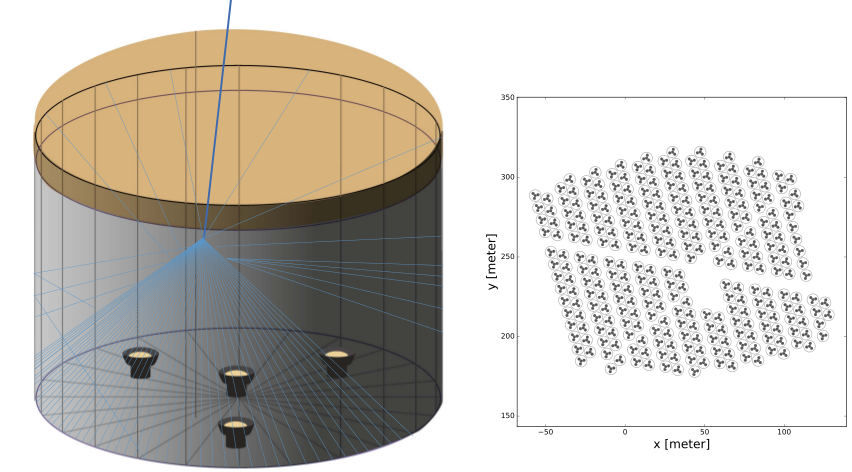
\includegraphics[scale = 0.3]{FIGURAS/TANQUE_HAWC.png}
		\caption{Lado izquierdo, esquema de un detector de agua Cherenkov. Lado derecho, esquema de distribución de los detectores en el observatorio HAWC \cite{Abeysekara}}.
		\label{TANQUE_HAWC}
	\end{figure}

	\subsection{Detectores Cherenkov}\label{DETECTORES_CHERENKOV}
		Los detectores Cherenkov de agua, o WCD por sus siglas en inglés Water Cherenkov Detector, han sido usados para la detección y construcción del espectro de CR's. Cada WCD tiene dimensiones de altura y diámetro variables dependiendo del observatorio; por ejemplo, Pierre Auger utiliza tanques de 1.55m de altura y 1.8m de diámetro. Un Tyvek reflectivo cubre internamente el tanque, el cual contiene agua purificada.
		
		\begin{figure}[h]
			\centering
			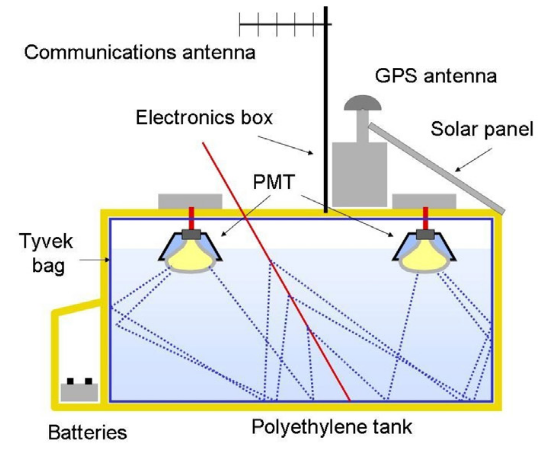
\includegraphics[scale = 0.5]{FIGURAS/TANQUE_CHERENKOV.png}
			\caption{Esquema de un WCD. Los fotones emitidos por las partículas cargadas al interacciones con el medio son detectados por los PMT \cite{LU2020163678}.}
			\label{TANQUE_CHERENKOV}
		\end{figure}
	
		Dentro del tanque además, se utilizan tubos fotomultiplicadores, o PMT's por sus siglas en inglés Photomultiplier Tubes, para la detección y amplificación de la señal de los fotones Cherenkov. Un amplificador es conectado en el último dínodo del PMT para una amplificación adicional a la señal. Los tanques pueden ser energéticamente autosuficientes usando paneles solares y baterias, además se puede manejar una sincronización temporal con la oficina central usando un GPS (Global Position System). Además, los datos pueden ser almacenados y procesados usando un micro-controlador para posteriormente ser enviados a la oficina central \cite{LU2020163678}. Dicho esquema de los WCD's se presenta en la fig. \ref{TANQUE_CHERENKOV}.